\documentclass{standalone}

\begin{document}
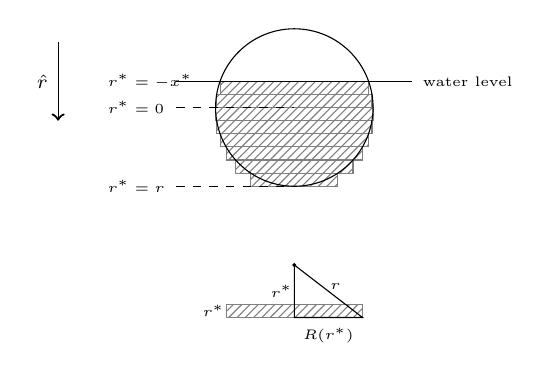
\begin{tikzpicture}

    \usetikzlibrary{decorations.pathreplacing,angles,quotes}
    \usetikzlibrary{shapes.geometric,shapes.misc}
    \usetikzlibrary{calc}
    \usetikzlibrary{patterns}



    \draw[->] (-3.0, 1/2) -- node[left] {\scriptsize $\hat r$} (-3.0, -1/2);

    \foreach \ra in {1/3, 1/6, 0, -1/6, -1/3, -1/2, -2/3, -5/6}
        \draw[gray, pattern = north east lines, pattern color = gray]
               ({sqrt(1-\ra*\ra)}, \ra-2/6)
            -- ({sqrt(1-\ra*\ra)}, \ra-3/6)
            -- ({-sqrt(1-\ra*\ra)}, \ra-3/6)
            -- ({-sqrt(1-\ra*\ra)}, \ra-2/6)
            -- cycle;

    \draw (-2.5, 0) node[right] {\tiny $r^* = -x^*$} (-1.5, 0)
        -- (1.5, 0) node[right] {\tiny water level};

    \draw (0, -2/6) circle (1);

    \draw[dashed] (-2.5, -2/6) node[right] {\tiny $r^* = 0$}
        (-1.5, -2/6) -- (0, -2/6);

    \draw[dashed] (-2.5, -8/6) node[right] {\tiny $r^* = r$}
        (-1.5, -8/6) -- (0, -8/6);

    % picture of one slice
    \draw[fill] (0, -2/6-2) circle (.5pt);

    \draw[gray, pattern = north east lines, pattern color = gray]
           ({sqrt(1-1/4)}, -1/2-2/6-2)
        -- ({sqrt(1-1/4)}, -1/2-3/6-2)
        -- ({-sqrt(1-1/4)}, -1/2-3/6-2)
        -- node[left=-3pt,black] {\tiny $\D r^*$} ({-sqrt(1-1/4)}, -1/2-2/6-2)
        -- cycle;

    \draw[black]
           (0, -1/3-2)
        -- node[above right=-3pt] {\tiny $r$} ({sqrt(1-1/4)}, -1/2-3/6-2)
        -- node[below] {\tiny $R(r^*)$} (0, -1/2-3/6-2)
        -- node[left=-3pt] {\tiny $r^*$} cycle;


\end{tikzpicture}
\end{document}
